
\documentclass[11pt,a4paper]{report}

\usepackage[a4paper,margin=1in]{geometry}
\usepackage{graphicx}
\graphicspath{{../}{../ActivityDiagram/}{../UseCaseDiagram/}{../ClassDiagram/}{../SequenceDiagram/}{../CollaborationDiagram/}{../StateDiagram/}{../ComponentDiagram/}{../DeploymentDiagram/}{../ObjectDiagram/}}
\usepackage{hyperref}
\usepackage{titlesec}
\usepackage{enumitem}
\usepackage{longtable}
\usepackage{array}
\usepackage{float}

\hypersetup{
colorlinks=true,
linkcolor=blue,
urlcolor=blue
}

\titleformat{\chapter}{\normalfont\LARGE\bfseries}{\thechapter.}{1em}{}

\begin{document}

% Cover and index remain as in original template

\begin{titlepage}
\centering

 
\includegraphics[width=0.7\textwidth]{thapar_logo.jpg}
\rule{0pt}{3cm}

\vspace{1cm}

{\Large \textbf{THAPAR INSTITUTE OF ENGINEERING AND TECHNOLOGY}}\\
{\large Department of Computer Science and Engineering}

\vspace{1.5cm}

{\Huge \textbf{Project Report Mid-Semester}}\\[0.5cm]
{\LARGE \textbf{Offline Hand Sign to Text Recognition System for American Sign Language}}

\vspace{1.5cm}

\textbf{Course Name \& Code:} UCS503 -- Software Engineering\\
\textbf{Degree \& Year:} B.Tech (3rd Year 3C18)\\
\textbf{Institute:} Thapar Institute of Engineering and Technology\\[0.5cm]

\textbf{Submitted To: Kirtika Goel}\\
\textbf{Submitted By:}\\
Keshav Aggarwal \hfill - 1024030234\\
Abhishek Srivastava \hfill - 1024030236\\
Harshine Singh \hfill - 1024030232\\
Bhuvaneesh Singh Grewal \hfill - 1024030235\\[1cm]

\textbf{Mid-Semester Evalution}\\
\textbf{Academic Year:} 2026--27 ODD SEMESTER

\vfill

\end{titlepage}

\tableofcontents
\newpage


\chapter{Introduction}

\section{Background and Context}

Communication between Deaf or Hard-of-Hearing individuals and people who do not understand American Sign Language (ASL) is a major accessibility challenge. Traditional communication requires either human interpreters or manual text conversion, which may not always be available.

This project proposes an offline, camera-based hand sign recognition system capable of converting ASL hand gestures into text in real time. The system uses a webcam to capture gestures, a React-based frontend for interaction, a Spring Boot backend for processing, and a Convolutional Neural Network (CNN) model trained using DeepLearning4J.

Unlike cloud-based solutions, all recognition operations occur locally, improving privacy, reducing latency, and removing dependency on external APIs.

\section{Problem Statement}

Many existing sign language recognition solutions rely on online services, external APIs, or specialized hardware. These limitations create problems related to cost, privacy, internet dependency, and accessibility.

The objective of this project is to develop a standalone software system that recognizes static ASL alphabet and digit signs (A-Z and 0-9) using only a standard webcam and local computational resources.

\section{Project Objectives}

\begin{enumerate}
\item Develop a real-time webcam based ASL sign recognition system.
\item Train a CNN model capable of classifying 36 ASL classes.
\item Establish communication between frontend and backend using WebSockets.
\item Provide text output corresponding to recognized signs.
\item Maintain complete offline operation without cloud AI services.
\item Provide support for future custom sign dictionary expansion.
\end{enumerate}


\chapter{Methodology and Design}

\section{System Architecture}

The system is divided into multiple layers:

\begin{itemize}
\item \textbf{User and Camera Layer:} Captures hand gestures using webcam input.
\item \textbf{React Frontend:} Processes frames, detects hand regions, resizes images and communicates with backend.
\item \textbf{Spring Boot Backend:} Receives frames through WebSocket communication and forwards them to the prediction module.
\item \textbf{CNN/DL4J Layer:} Loads the trained CNN model, performs feature extraction and classification.
\item \textbf{Training Pipeline:} Performs preprocessing, dataset splitting and CNN training.
\end{itemize}


\section{UML System Design and Architectural Modeling}

The system architecture and behavior are formally specified using the complete suite of Unified Modeling Language (UML) design models conforming to IEEE and software engineering standards.

\subsection{Use Case Diagram}
The Use Case Diagram defines actor interactions, system boundaries, and functional requirements across three operational packages: runtime live recognition, REST API word assistance, and offline dataset training. The primary actors include the end user (signer), webcam device, ML engineer, data engineer, and local storage systems.

\begin{figure}[H]
\centering
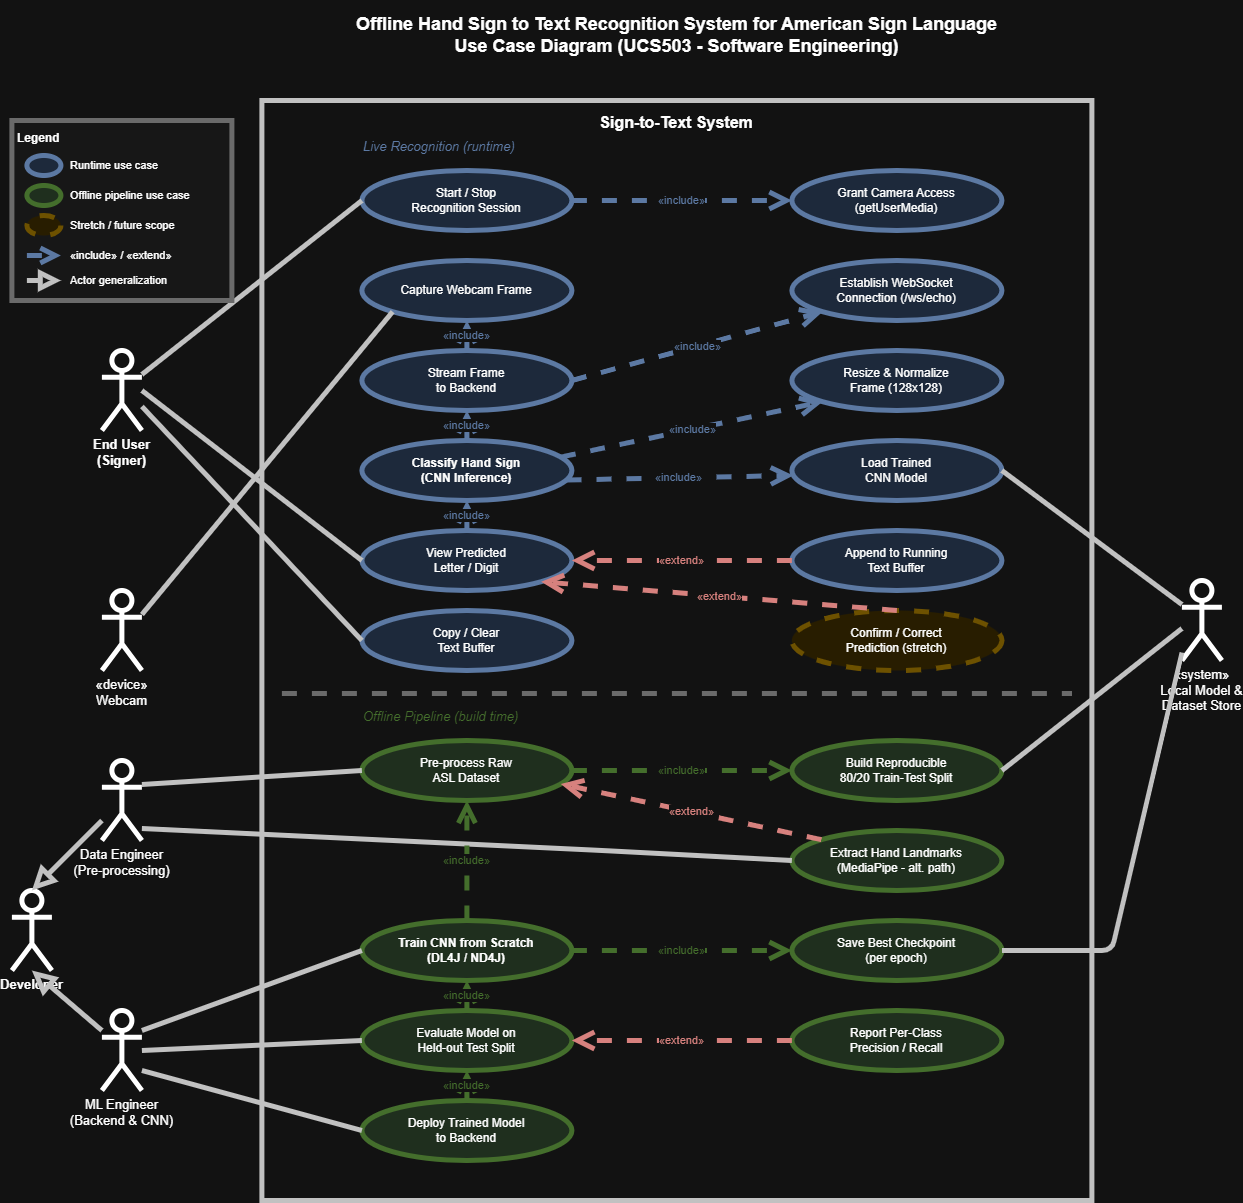
\includegraphics[width=\textwidth]{UseCaseDiagram.png}
\caption{Use Case Diagram of Sign-to-Text Recognition System}
\end{figure}

\subsection{Activity Diagrams}
The Activity Diagrams model concurrent workflows and decision logic across two distinct lifecycles:
\begin{enumerate}
    \item \textbf{Live ASL Recognition:} Swimlane-partitioned workflow across User, React Frontend, and Spring Boot Backend, illustrating 350~ms canvas capture, Base64 decoding, in-process DL4J inference, confidence thresholding ($\ge 0.85$), and 4-frame streak commit.
    \item \textbf{Model Training Pipeline:} Offline training workflow detailing image preprocessing, 80/20 train-test splitting (seed 42), DL4J CNN epoch iterations, validation evaluation, and model artifact serialization.
\end{enumerate}

\begin{figure}[H]
\centering
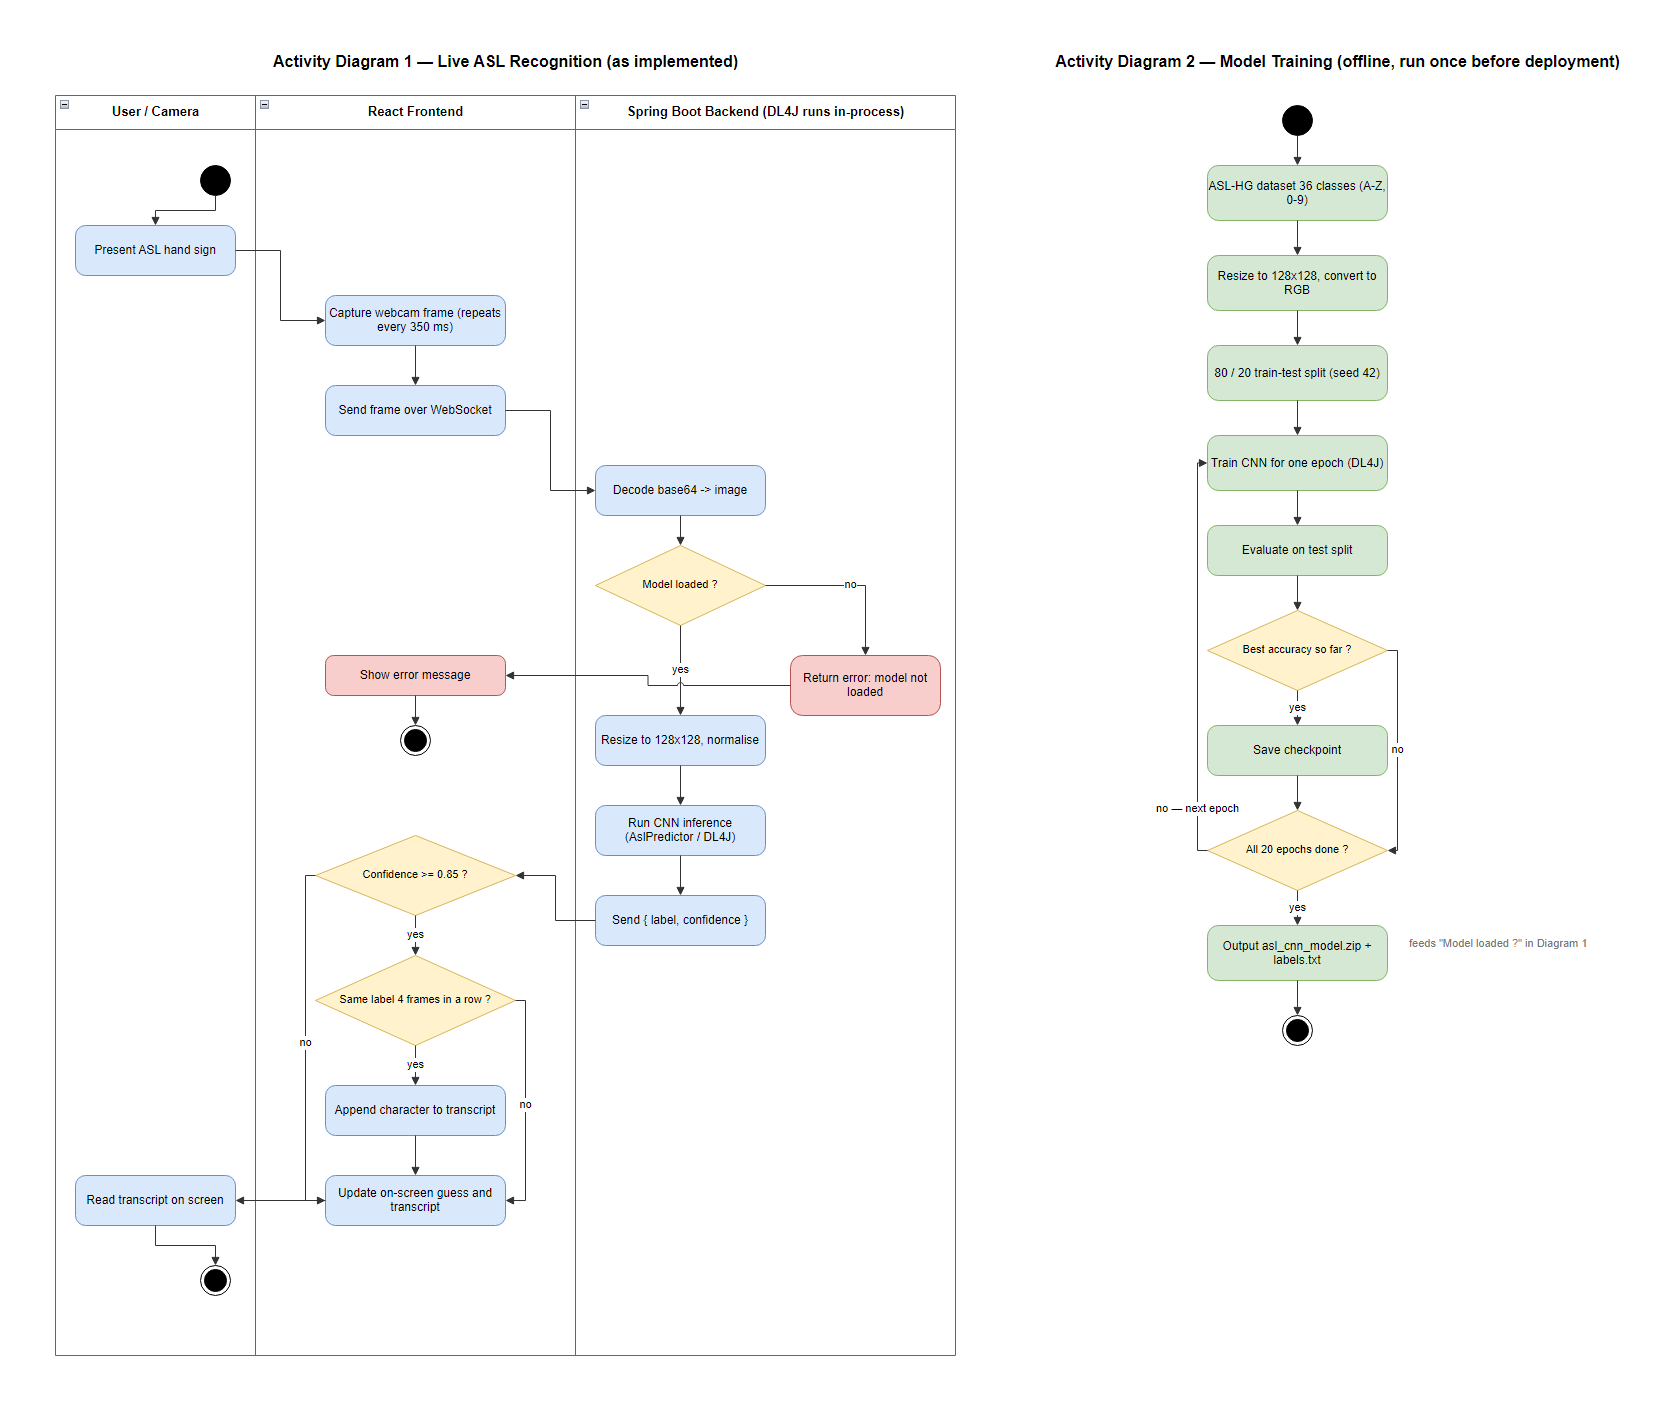
\includegraphics[width=\textwidth]{ActivityDiagram.png}
\caption{Activity Diagram: Real-Time Live Recognition and Offline Training Workflows}
\end{figure}

\subsection{Class Diagram}
The Class Diagram models all object-oriented structures, class hierarchies, interfaces, fields, methods, and layer boundaries across the Spring Boot backend. It includes configuration classes (\texttt{WebSocketConfig}), boundaries (\texttt{AslWebSocketHandler}, \texttt{SystemApiController}, \texttt{DictionaryController}), services (\texttt{TranscriptStabilizerService}, \texttt{DictionaryService}), machine learning wrappers (\texttt{AslPredictor}, \texttt{AslCnnModel}), persistence entities and repositories (\texttt{TranslationSession}, \texttt{TranslationSessionRepository}), and immutable DTO records.

\begin{figure}[H]
\centering
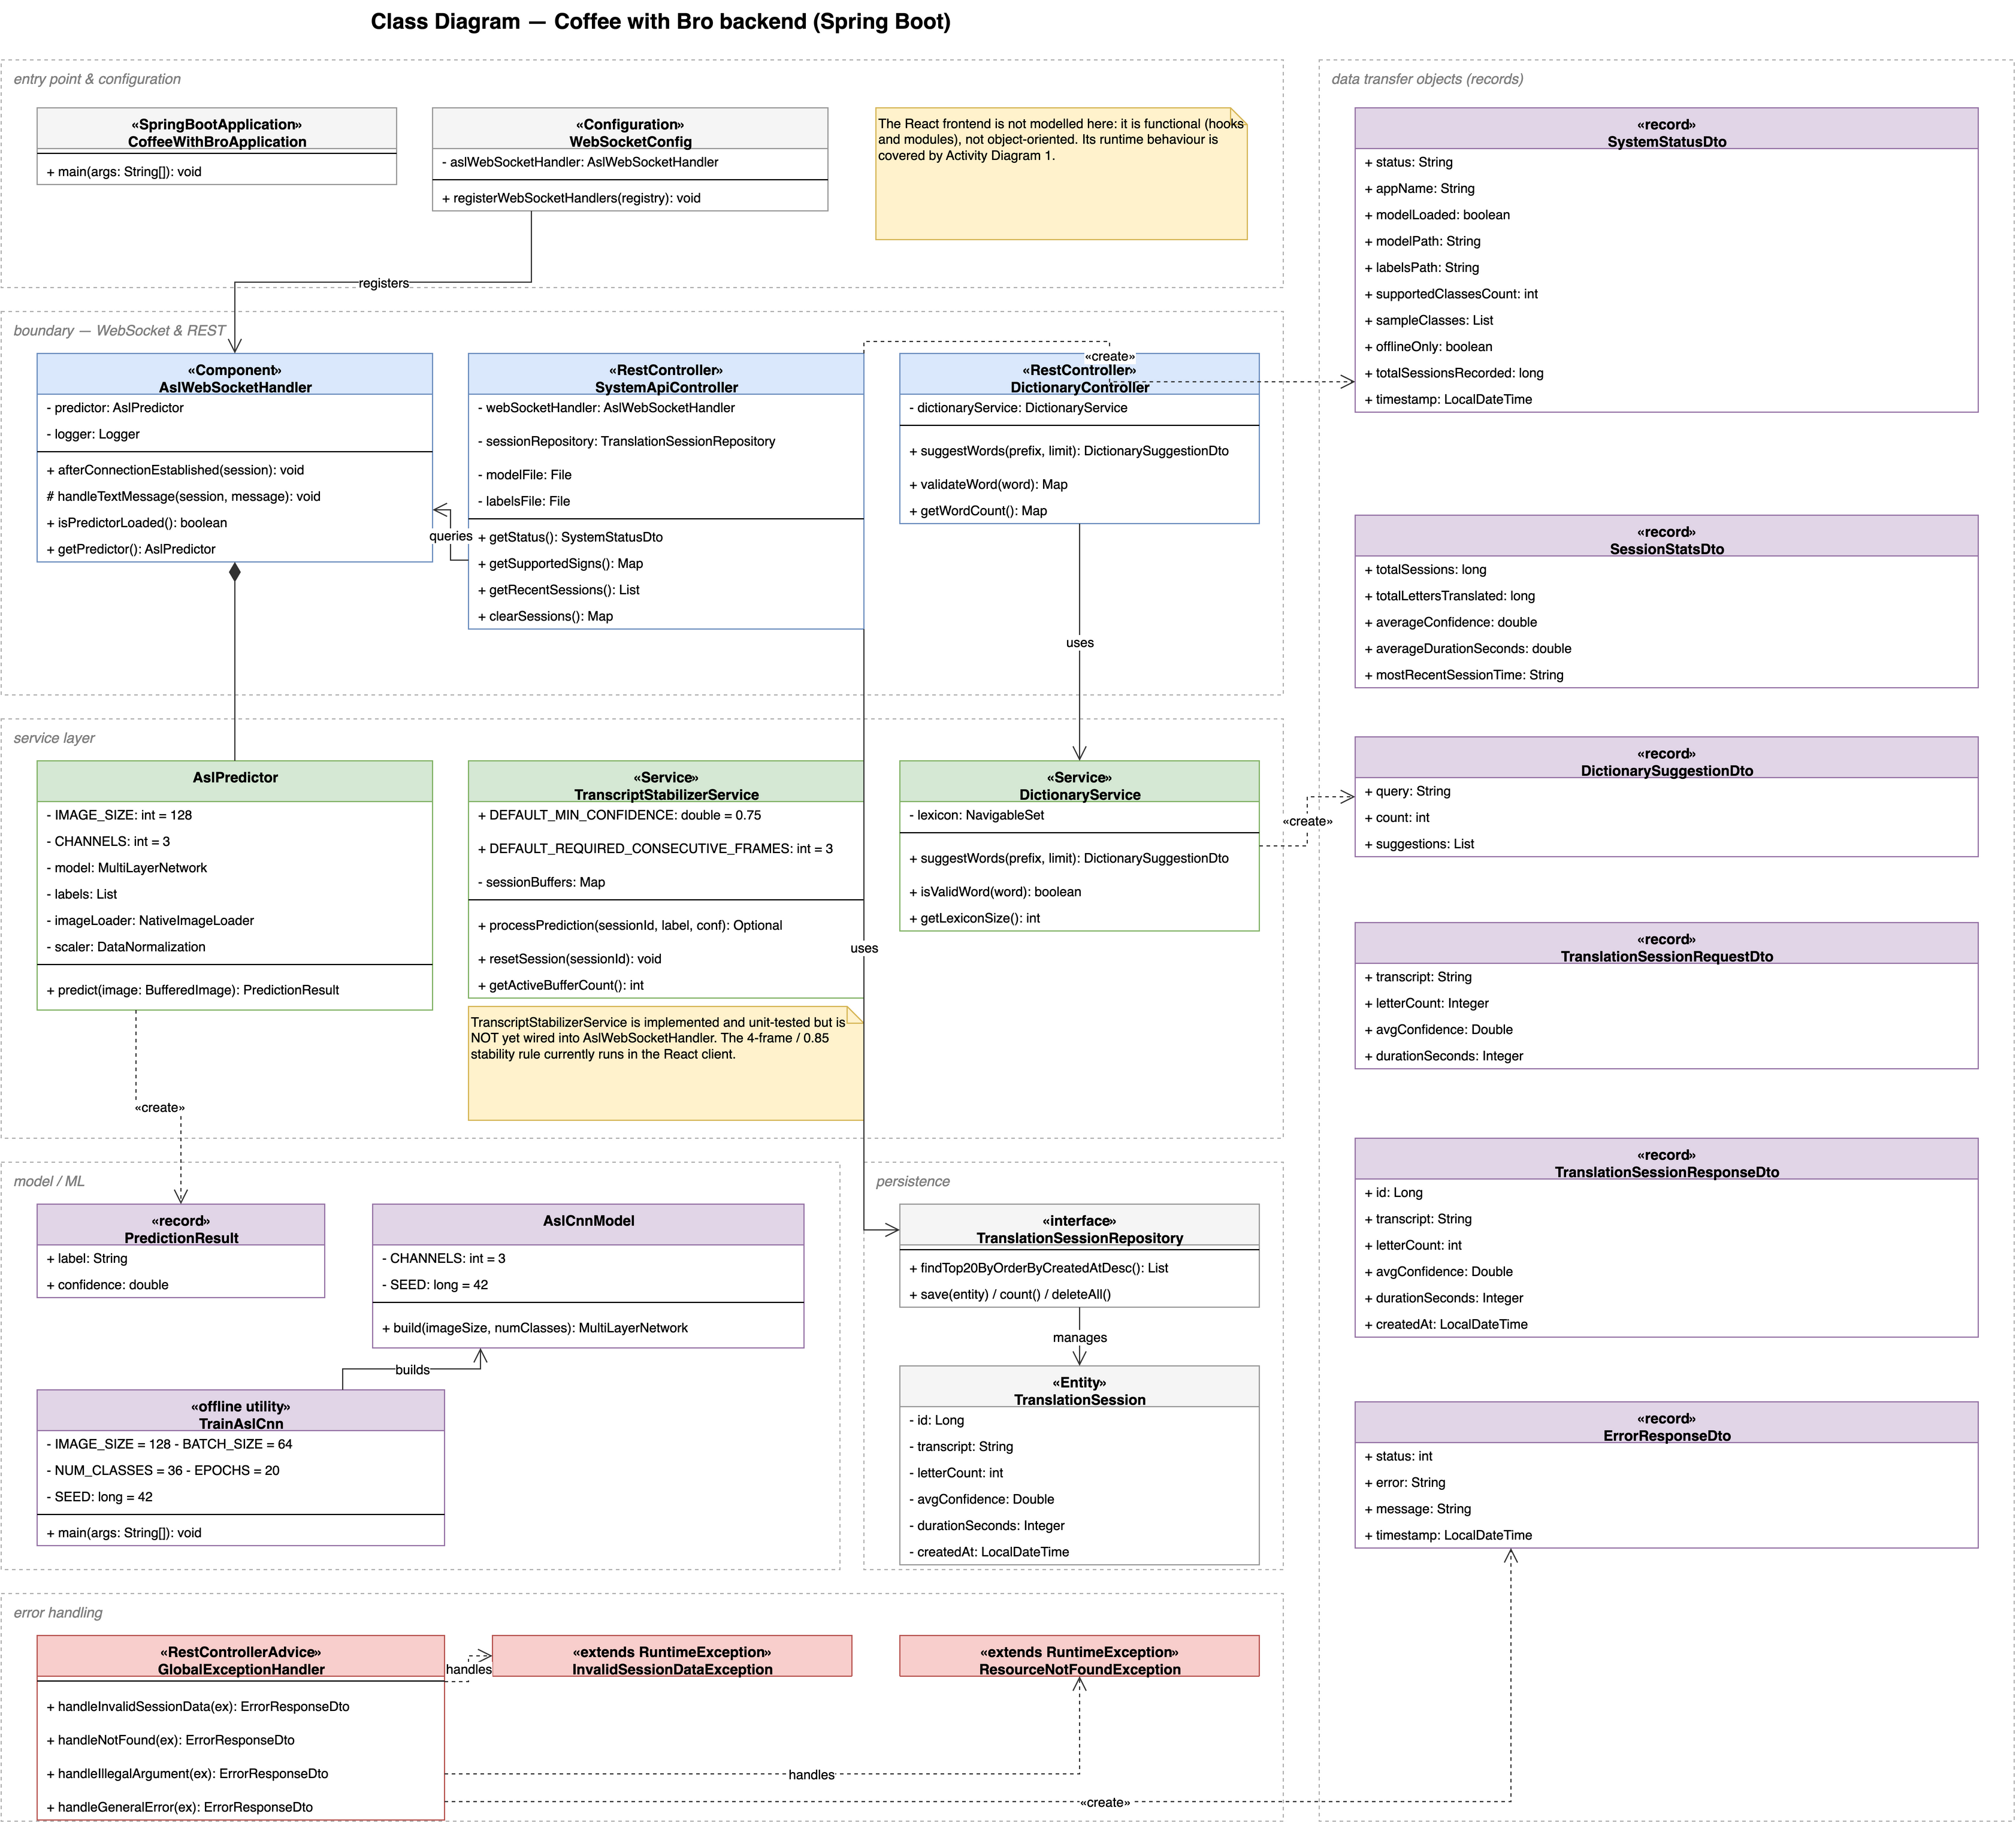
\includegraphics[width=\textwidth]{ClassDiagram.png}
\caption{UML Class Diagram of Backend Service Architecture}
\end{figure}

\subsection{Sequence Diagram}
The Sequence Diagram details the chronological message protocols between participating lifelines during live execution and offline model generation. It explicitly details the 350~ms frame grab loop, Base64 transmission over \texttt{ws://localhost:8080/ws/echo}, in-process ND4J matrix normalization, prediction response handling, consecutive streak accumulation, prefix autocomplete queries, and H2 database session persistence.

\begin{figure}[H]
\centering
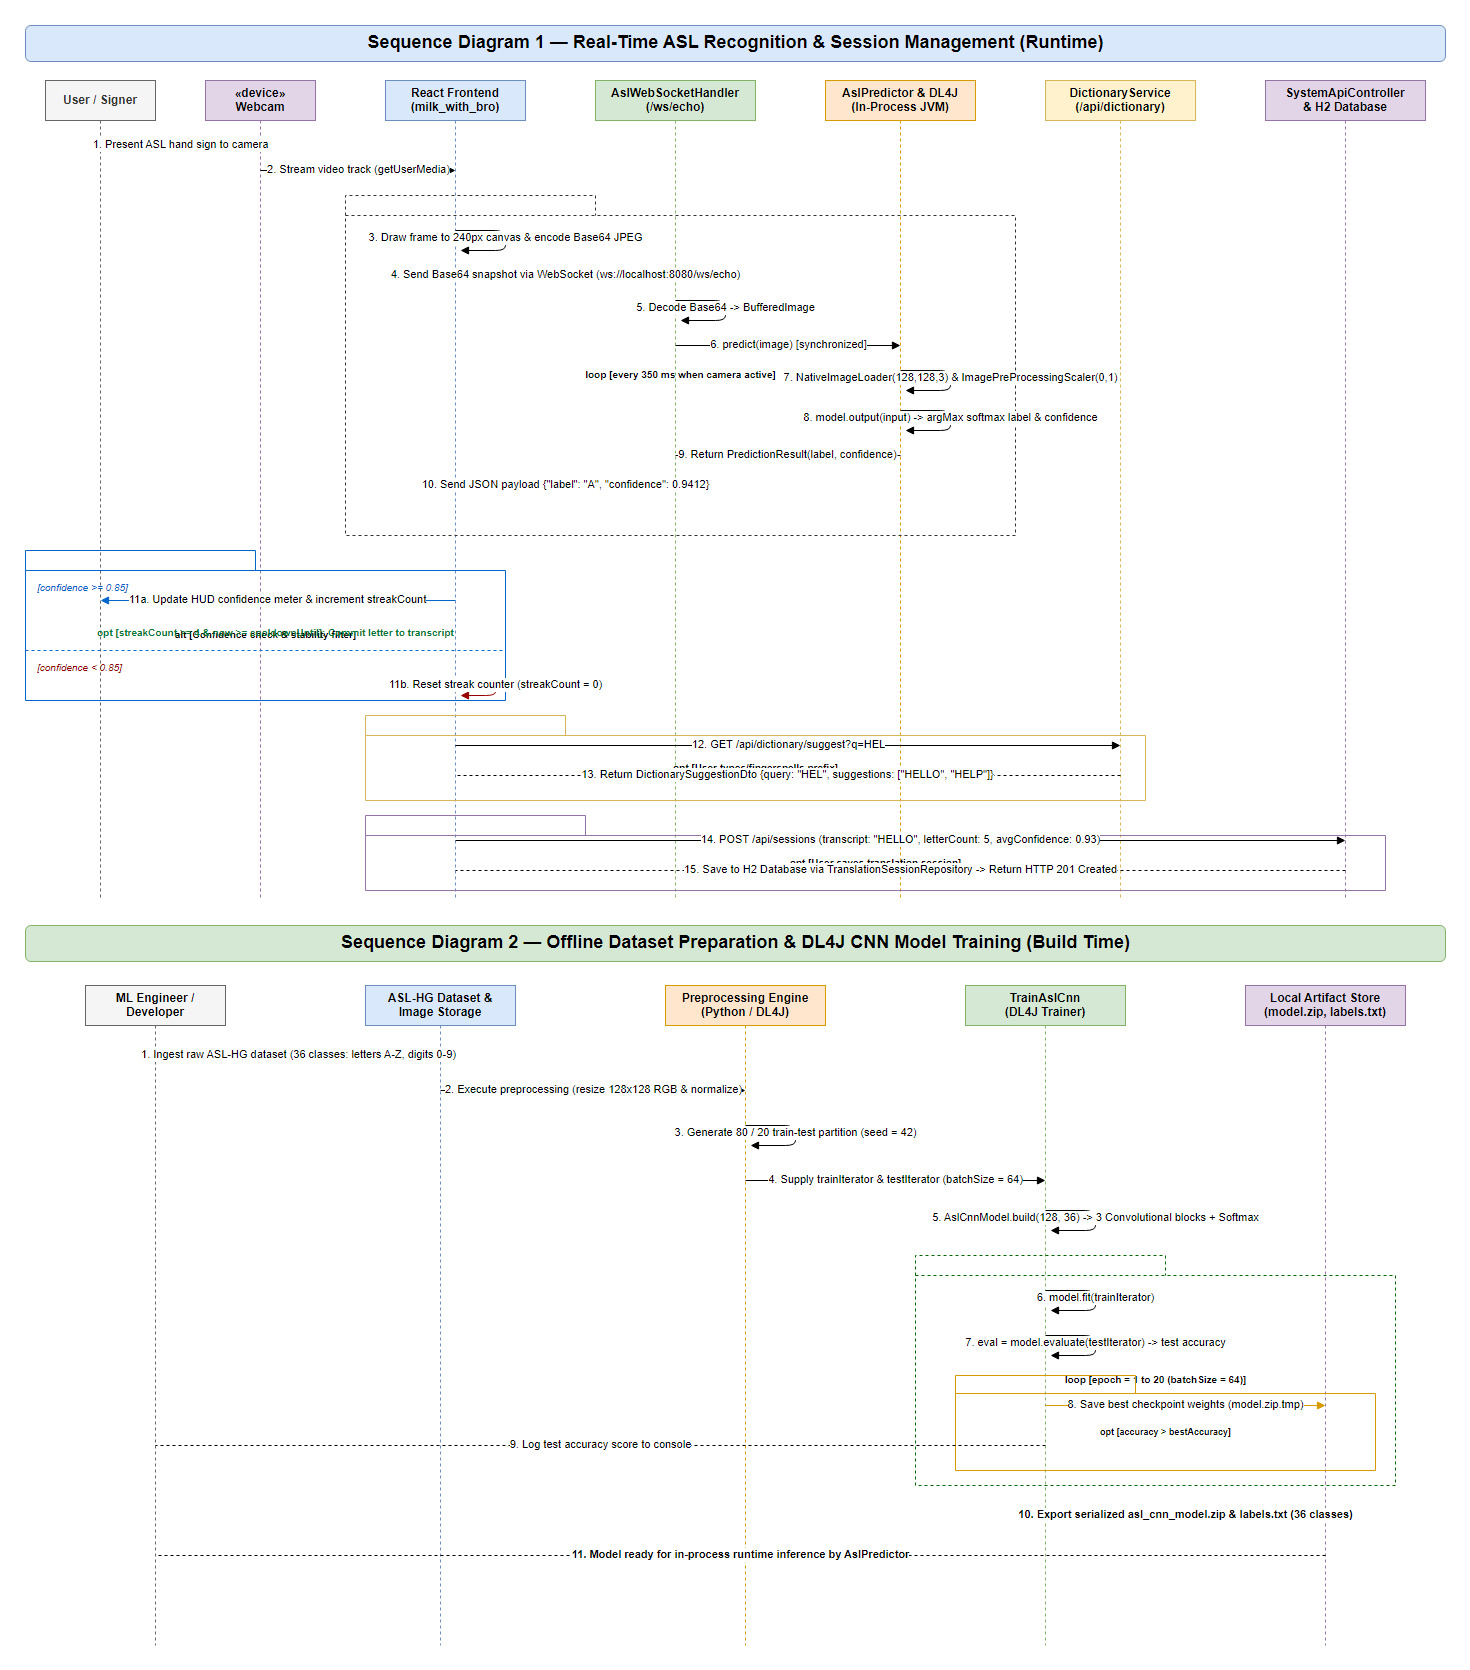
\includegraphics[width=\textwidth]{SequenceDiagram.png}
\caption{Sequence Diagram of Real-Time Recognition and Offline Training Lifelines}
\end{figure}

\subsection{Collaboration / Communication Diagram}
The Collaboration Diagram illustrates object associations, structural links, and numbered message flows among collaborating runtime instances, demonstrating the decoupled relationship between client-side capture, in-process DL4J neural computation, and embedded database storage.

\begin{figure}[H]
\centering
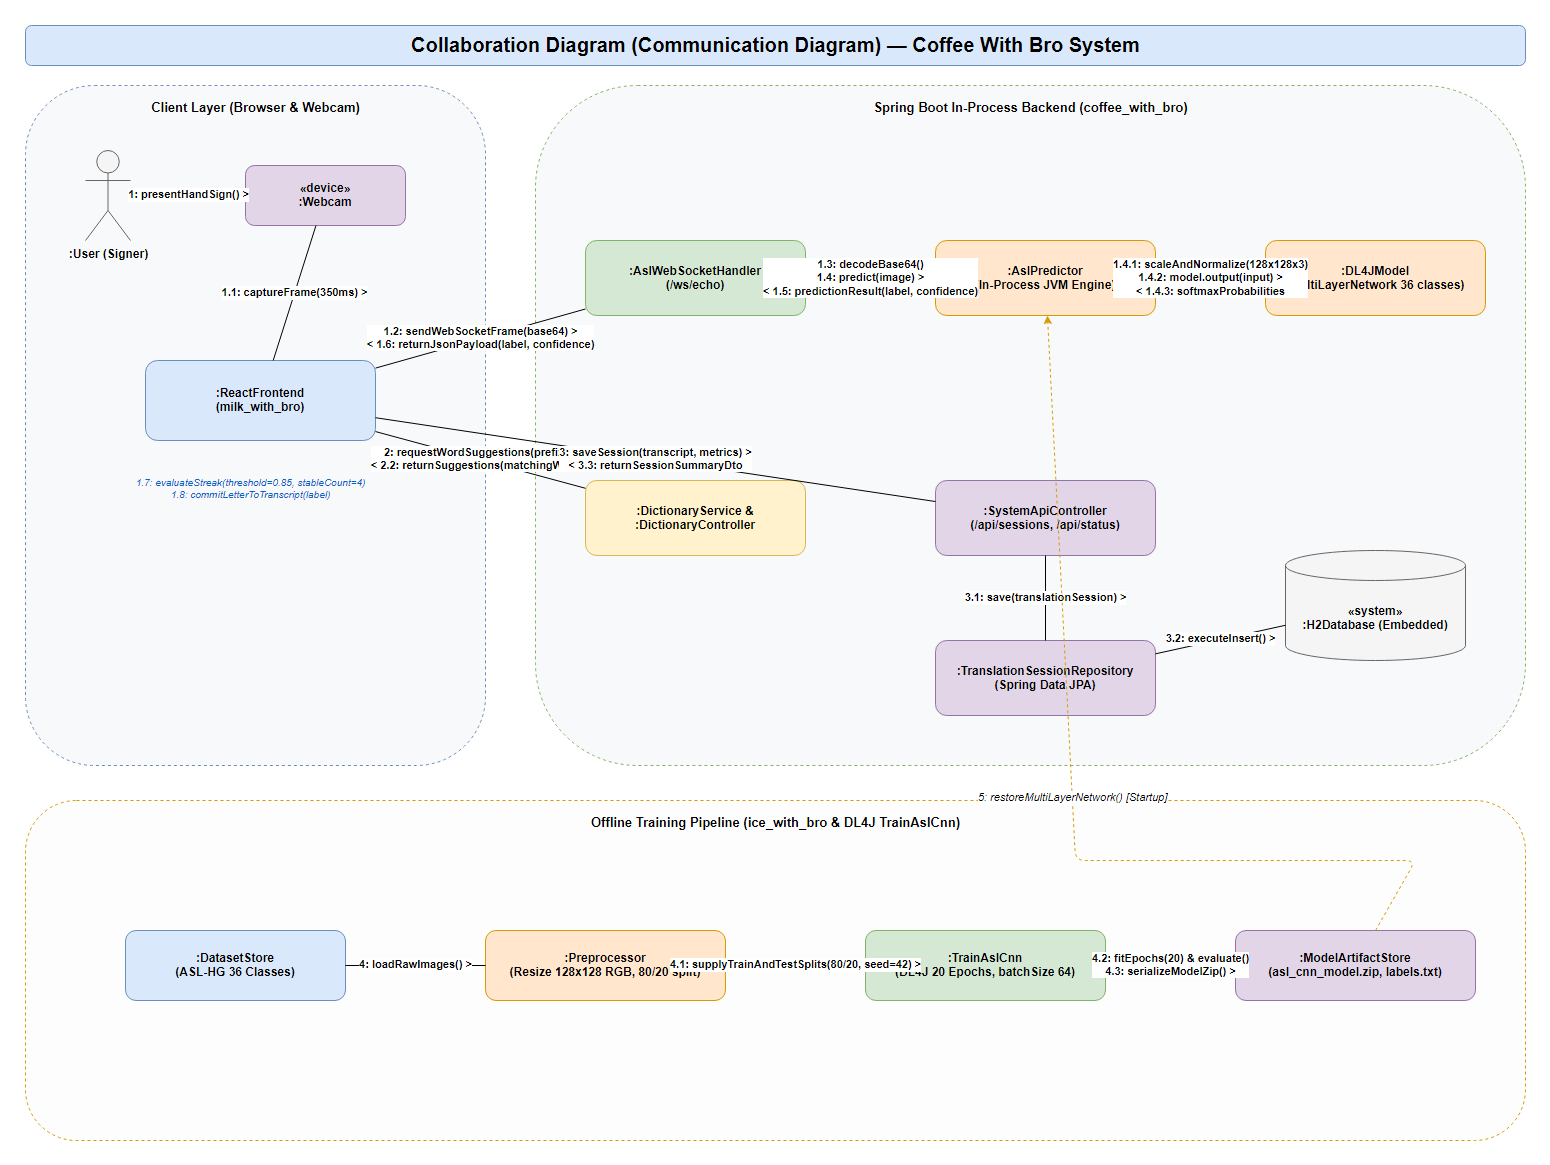
\includegraphics[width=\textwidth]{CollaborationDiagram.png}
\caption{Collaboration Diagram (Communication Diagram) of System Instances}
\end{figure}

\subsection{State Machine Diagram}
The State Machine Diagram formalizes system states, transitions, guard conditions, and actions throughout the client application lifecycle, from initial standby and WebSocket handshakes, through the streaming/inference superstate, streak accumulation, and transcript letter commit, to dictionary queries and session persistence.

\begin{figure}[H]
\centering
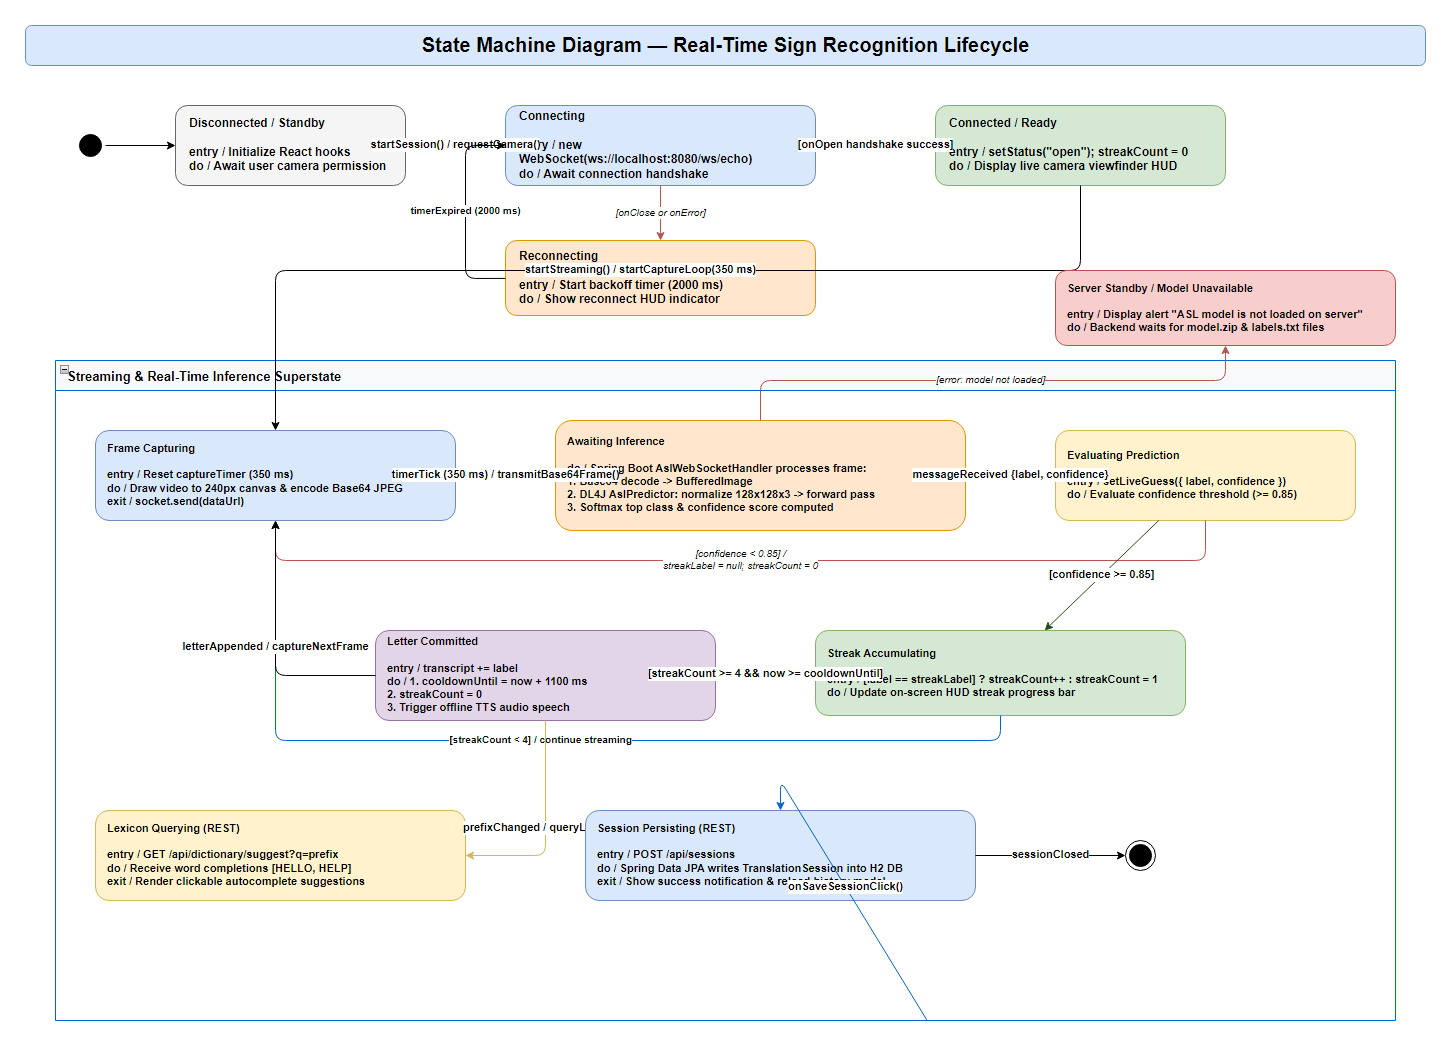
\includegraphics[width=\textwidth]{StateDiagram.png}
\caption{State Machine Diagram of Recognition and Client Lifecycle}
\end{figure}

\subsection{Component Diagram}
The Component Diagram details the modular decomposition of the architecture into the React 19 Frontend (viewfinder, WebSocket client, transcript builder, HUD), Spring Boot Backend (WebSocket handler, DL4J inference engine, lexicon service, REST controllers), Data Tier (embedded H2 database, local model store), and Offline Training Pipeline, highlighting provided and required interface ports.

\begin{figure}[H]
\centering
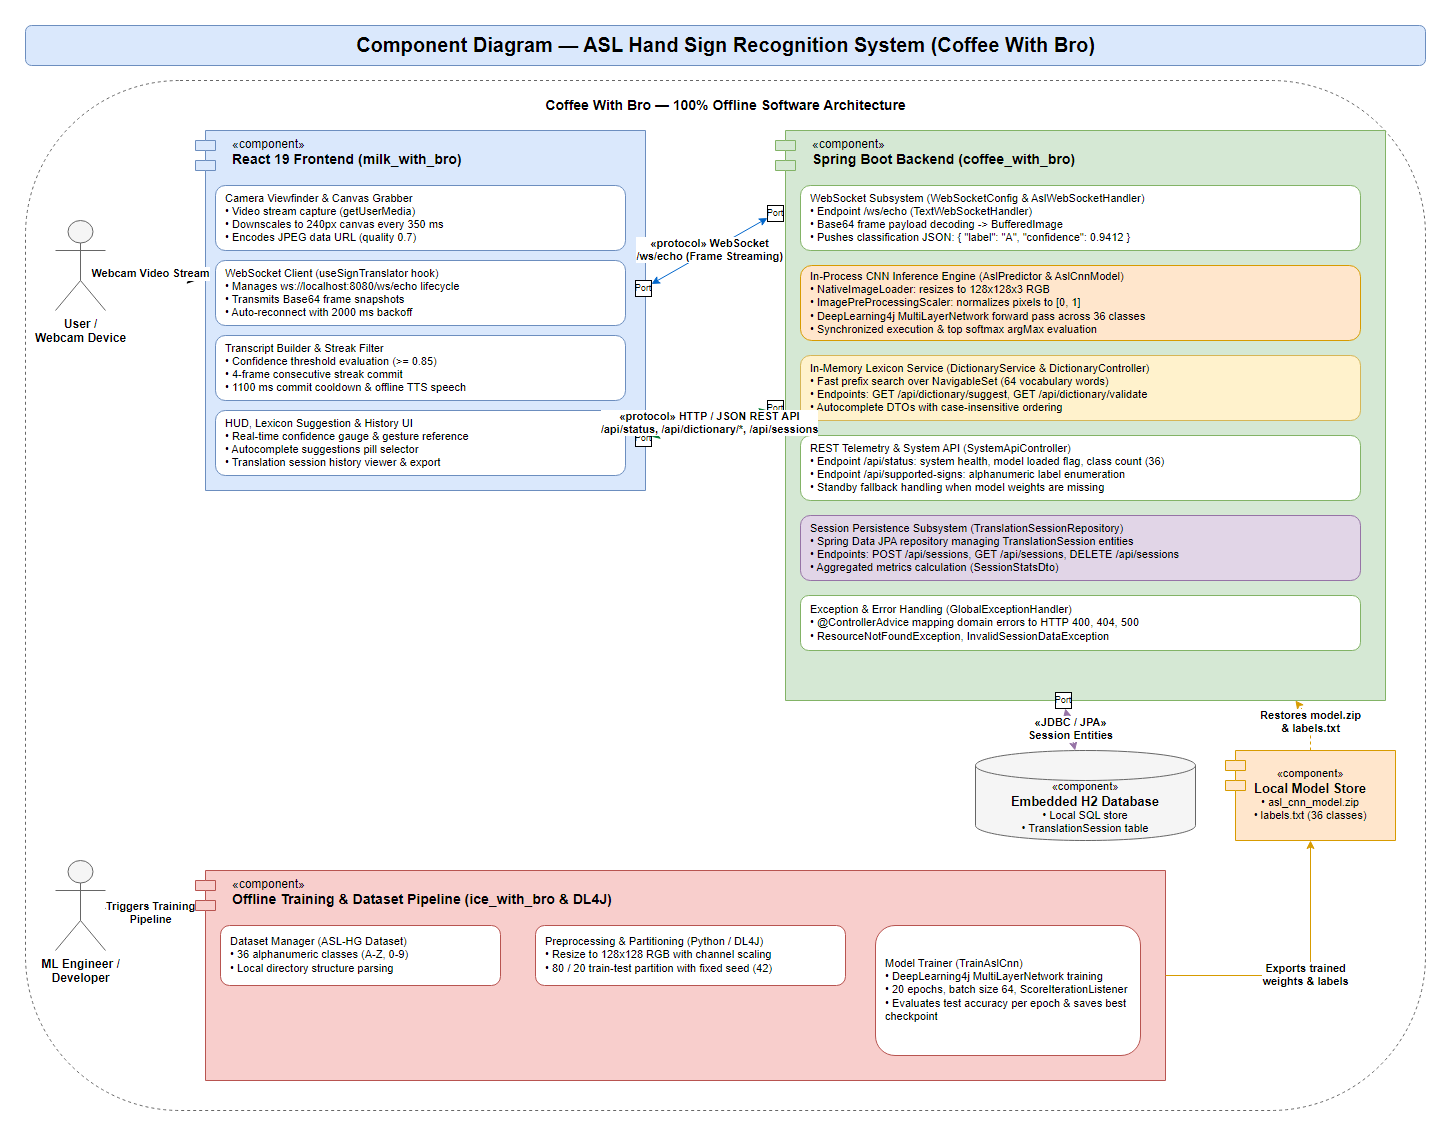
\includegraphics[width=\textwidth]{ComponentDiagram.png}
\caption{Component Diagram of Modular Subsystem Architecture and Ports}
\end{figure}

\subsection{Deployment Diagram}
The Deployment Diagram models the physical workstation device, execution environments (V8 Browser, JDK 17 JVM, Host File System), and deployed artifacts. It formally documents the 100\% offline, zero-cloud execution model that ensures total privacy and instant local inference.

\begin{figure}[H]
\centering
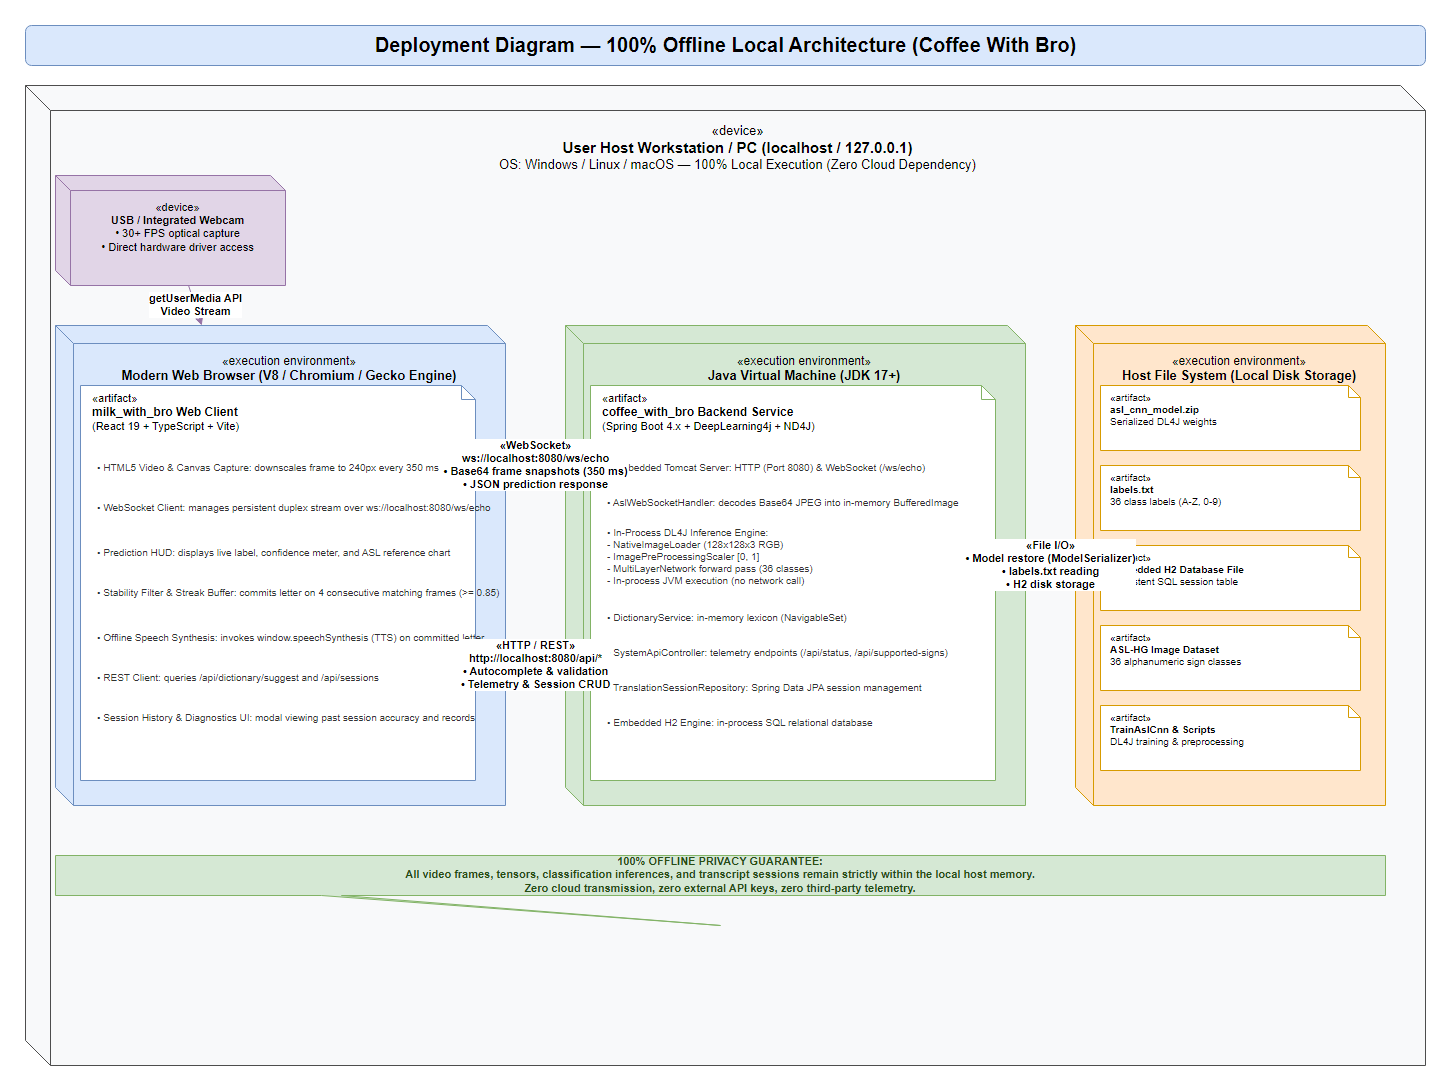
\includegraphics[width=\textwidth]{DeploymentDiagram.png}
\caption{Deployment Diagram of 100\% Offline Local Workstation Architecture}
\end{figure}

\subsection{Object Diagram}
The Object Diagram provides a concrete runtime snapshot captured one frame after classification of a gesture, showing live instance memory allocations, attribute values, and inter-object references across WebSocket sessions, handler instances, prediction records, client streak buffers, and JPA repositories.

\begin{figure}[H]
\centering
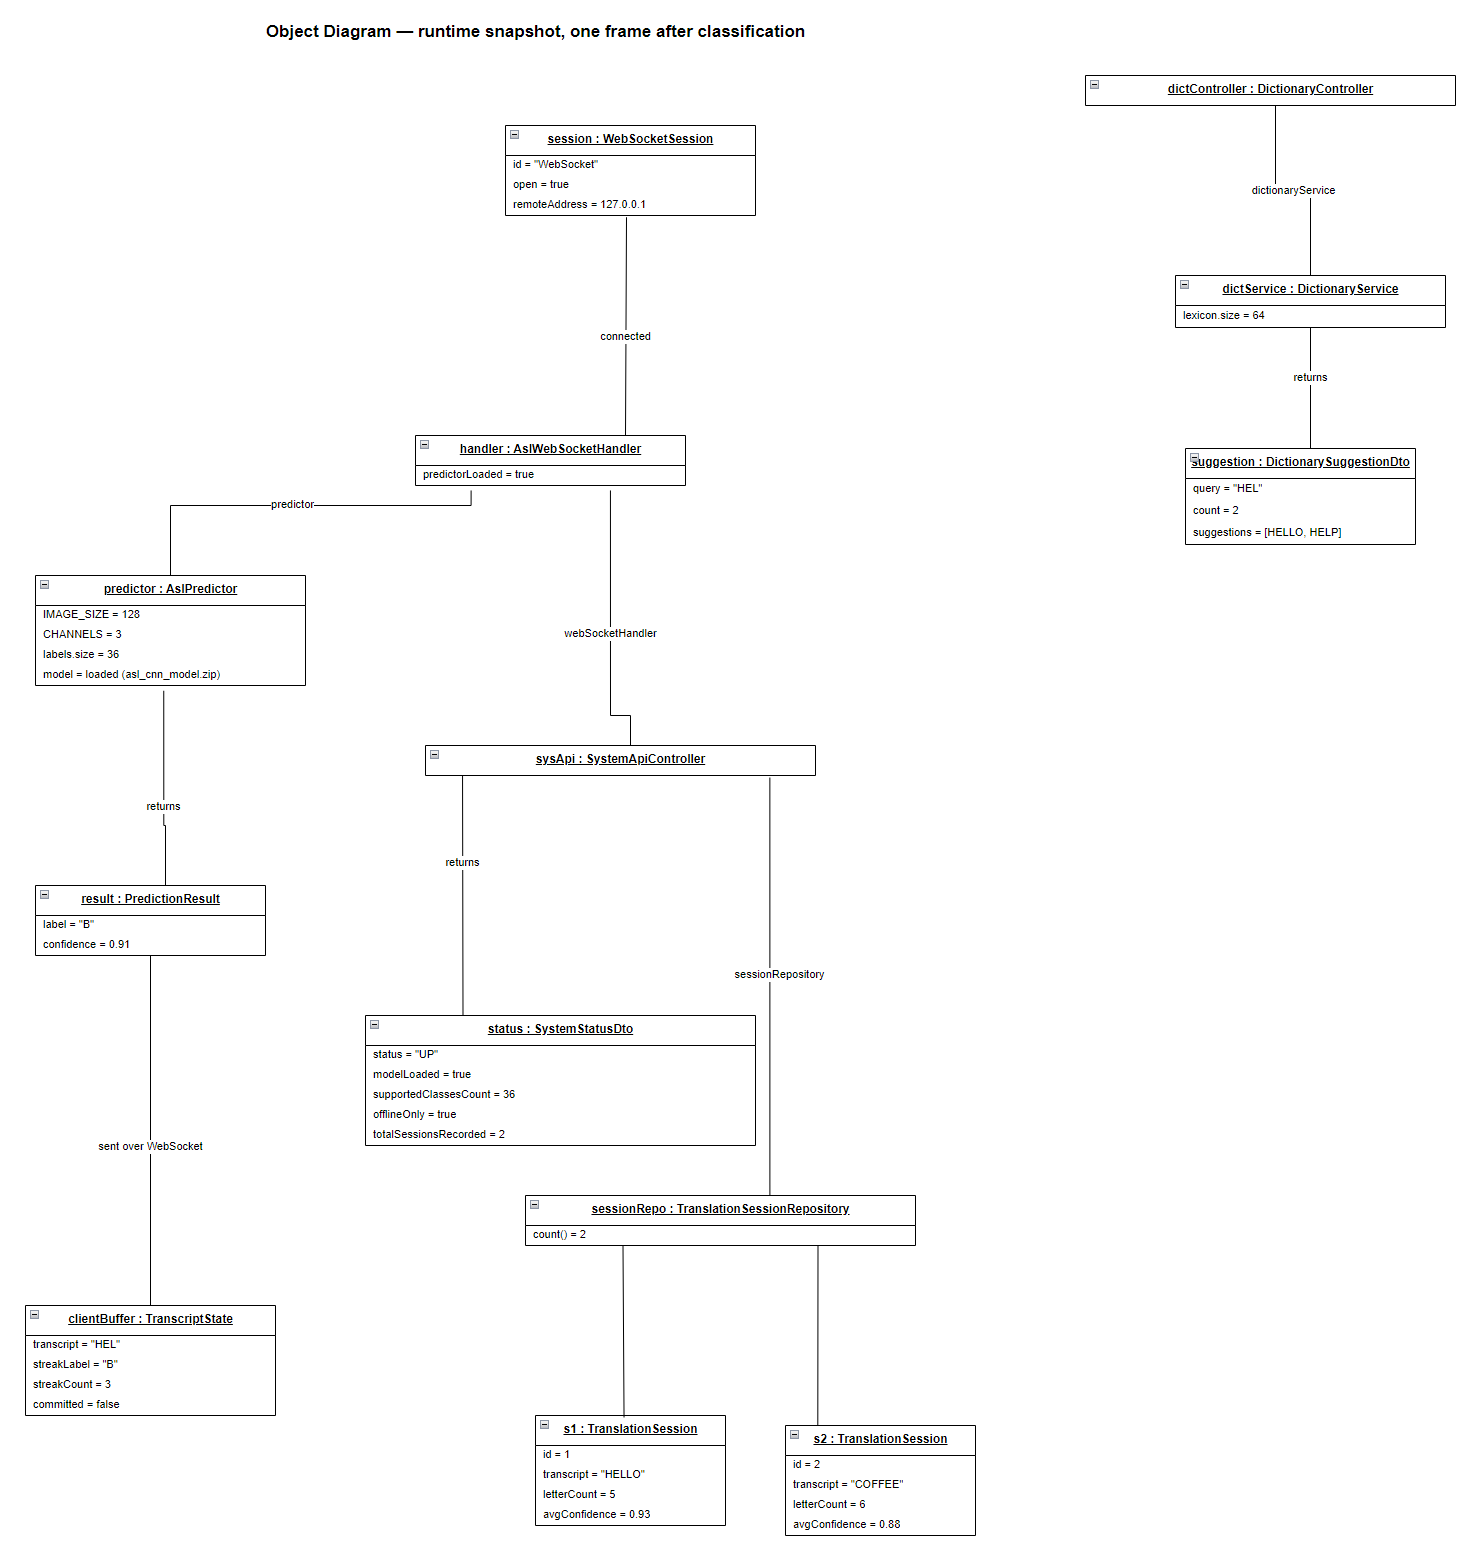
\includegraphics[width=\textwidth]{ObjectDiagram.png}
\caption{Object Diagram Runtime Snapshot One Frame After Classification}
\end{figure}


\section{Technical Stack}

\begin{itemize}
\item Frontend: React, TypeScript, Vite
\item Backend: Java 17 (LTS), Spring Boot 4.x
\item Machine Learning: DeepLearning4J, ND4J, DataVec
\item Communication: WebSocket
\item Build System: Maven
\item Dataset Processing: Python preprocessing scripts
\end{itemize}


\section{Implementation Details}

\subsection{CNN Based Recognition Module}

The CNN model consists of three convolution blocks with filter sizes 32, 64 and 128. Each block contains convolution, batch normalization, ReLU activation and max pooling operations.

The input image size is 128x128 RGB. Images are normalized before being passed to the CNN. The final layers consist of a dense layer followed by dropout and a softmax classifier.

\subsection{Frontend Recognition and Accessibility Module}

The frontend captures webcam frames continuously. Frames are processed and transmitted to the backend through WebSocket communication. Received predictions contain the recognized label and confidence score. The interface features a real-time HUD with confidence meters, an offline Speech Synthesis engine (Text-to-Speech) for acoustic readout of recognized signs, an interactive 36-class ASL sign reference guide, and session history management.

\subsection{Backend Prediction and Telemetry Module}

The Spring Boot backend loads the trained CNN model and label mapping. The predictor converts received images into tensors, performs inference and returns the predicted sign over WebSocket. Additionally, a REST API layer (`/api/status`, `/api/supported-signs`, `/api/sessions`) provides live telemetry and persists translation history into an embedded H2 database via Spring Data JPA.

\subsection{Custom Dictionary Extension}

The system supports future extension through a custom dictionary mechanism where users can add new gestures by collecting samples and associating them with user-defined labels.


\chapter{Results and Evaluation}

\section{Testing Methodology}

The system evaluation includes:

\begin{itemize}
\item Unit testing of backend components.
\item Integration testing between React frontend and Spring Boot backend.
\item CNN model testing on unseen images.
\item Performance evaluation of prediction latency.
\end{itemize}

\section{Performance Metrics}

\begin{table}[H]
\centering
\begin{tabular}{|c|c|}
\hline
Metric & Description\\
\hline
Classes Supported & 36 ASL classes\\
Image Size & 128x128 RGB\\
Inference & Local execution\\
Communication & WebSocket\\
Model Type & CNN\\
\hline
\end{tabular}
\caption{System Performance Metrics}
\end{table}


\section{Analysis}

The developed system successfully establishes an end-to-end sign recognition pipeline. The integration of computer vision, deep learning and web technologies provides a practical offline communication solution.

The main challenges include dataset variation, lighting conditions and maintaining prediction accuracy across different users.


\chapter{Conclusion}

\section{Summary of Work}

This project presents an offline American Sign Language recognition system that converts static hand gestures into text using a CNN model deployed through a Spring Boot backend.

\section{Key Findings}

\begin{itemize}
\item Local inference improves privacy and eliminates API dependency.
\item WebSocket communication enables real-time interaction.
\item CNN based classification provides an efficient recognition approach.
\item The architecture allows future expansion through custom vocabulary support.
\end{itemize}

\section{Future Work and Recommendations}

Future improvements include:

\begin{enumerate}
\item Recognition of dynamic word-level gestures.
\item Larger ASL vocabulary support.
\item Improved accuracy using additional datasets.
\item Mobile and edge-device deployment.
\item Advanced personalized sign learning.
\end{enumerate}


\chapter*{Bibliography}

\begin{enumerate}

\item Software Requirements Specification (SRS) document for Offline Hand Sign to Text Recognition System.

\item Activity Diagram and Use Case Diagram documentation created for UCS503 Software Engineering project.

\item ASL Hand Gesture Dataset:
\url{https://data.mendeley.com/datasets/j4y5w2c8w9/1}

\item DeepLearning4J Documentation.

\item Spring Boot Documentation.

\end{enumerate}


\end{document}
